\documentclass[landscape,a3paper]{article}
\usepackage[margin=1.2cm]{geometry}
\usepackage{tikz}
\usepackage[T1]{fontenc}
\usepackage[utf8]{inputenc}
\usepackage{helvet}
\renewcommand{\familydefault}{\sfdefault}
\usepackage{amsmath}
\usepackage{xcolor}
\usepackage{calc}

\usetikzlibrary{
  shapes.geometric,
  shapes.symbols,
  arrows.meta,
  positioning,
  fit,
  backgrounds,
  decorations.pathreplacing,
  shadows
}

\definecolor{OfflineBlue}{RGB}{220,232,245}
\definecolor{OfflineBorder}{RGB}{91,130,185}
\definecolor{OnlineGreen}{RGB}{220,245,228}
\definecolor{OnlineBorder}{RGB}{60,160,90}
\definecolor{InputColor}{RGB}{255,245,200}
\definecolor{InputBorder}{RGB}{210,160,0}
\definecolor{AlgaeColor}{RGB}{180,230,160}
\definecolor{AlgaeBorder}{RGB}{60,150,40}
\definecolor{AlgaeDark}{RGB}{30,110,20}
\definecolor{CrustColor}{RGB}{255,215,155}
\definecolor{CrustBorder}{RGB}{210,120,20}
\definecolor{CrustDark}{RGB}{160,80,0}
\definecolor{FishColor}{RGB}{180,215,250}
\definecolor{FishBorder}{RGB}{50,110,200}
\definecolor{FishDark}{RGB}{20,70,160}
\definecolor{ProcessGray}{RGB}{240,240,245}
\definecolor{ProcessBorder}{RGB}{130,130,160}
\definecolor{DBColor}{RGB}{235,225,255}
\definecolor{DBBorder}{RGB}{120,80,200}
\definecolor{OutputColor}{RGB}{255,230,230}
\definecolor{OutputBorder}{RGB}{200,60,60}
\definecolor{RiskRed}{RGB}{200,40,40}
\definecolor{RiskAmber}{RGB}{210,140,0}
\definecolor{RiskGreenC}{RGB}{40,150,50}

\tikzset{
  arr/.style={-{Stealth[length=7pt,width=5pt]}, line width=1.2pt, color=#1},
  arr/.default=black,
  proc/.style={
    rectangle, rounded corners=3pt,
    draw=#1!80!black, line width=1.1pt,
    fill=#1, text=black,
    font=\footnotesize\sffamily,
    text width=3.6cm, align=center,
    minimum height=0.8cm, inner sep=4pt
  },
  data/.style={
    trapezium, trapezium left angle=80, trapezium right angle=100,
    draw=#1!80!black, line width=1.1pt,
    fill=#1, text=black,
    font=\footnotesize\sffamily,
    text width=3.2cm, align=center,
    minimum height=0.75cm, inner sep=4pt
  },
  db/.style={
    cylinder, shape border rotate=90,
    draw=DBBorder, line width=1.1pt,
    fill=DBColor, text=black,
    font=\footnotesize\sffamily,
    text width=2.8cm, align=center,
    minimum height=1.0cm, aspect=0.25, inner sep=3pt
  },
  dec/.style={
    diamond, draw=ProcessBorder, line width=1.1pt,
    fill=ProcessGray, text=black,
    font=\scriptsize\sffamily,
    text width=2.0cm, align=center,
    minimum height=0.9cm, aspect=1.8, inner sep=2pt
  },
  seclabel/.style={font=\small\bfseries\sffamily, text=#1}
}

\pagestyle{empty}

\begin{document}
\begin{center}

{\LARGE\bfseries\sffamily TaxoTox --- Architectural Workflow}\\[3pt]
{\normalsize\sffamily Mixture Toxicity Assessment of Aquatic Pollutant Assemblages using the Toxic Unit (TU) Framework}\\[6pt]

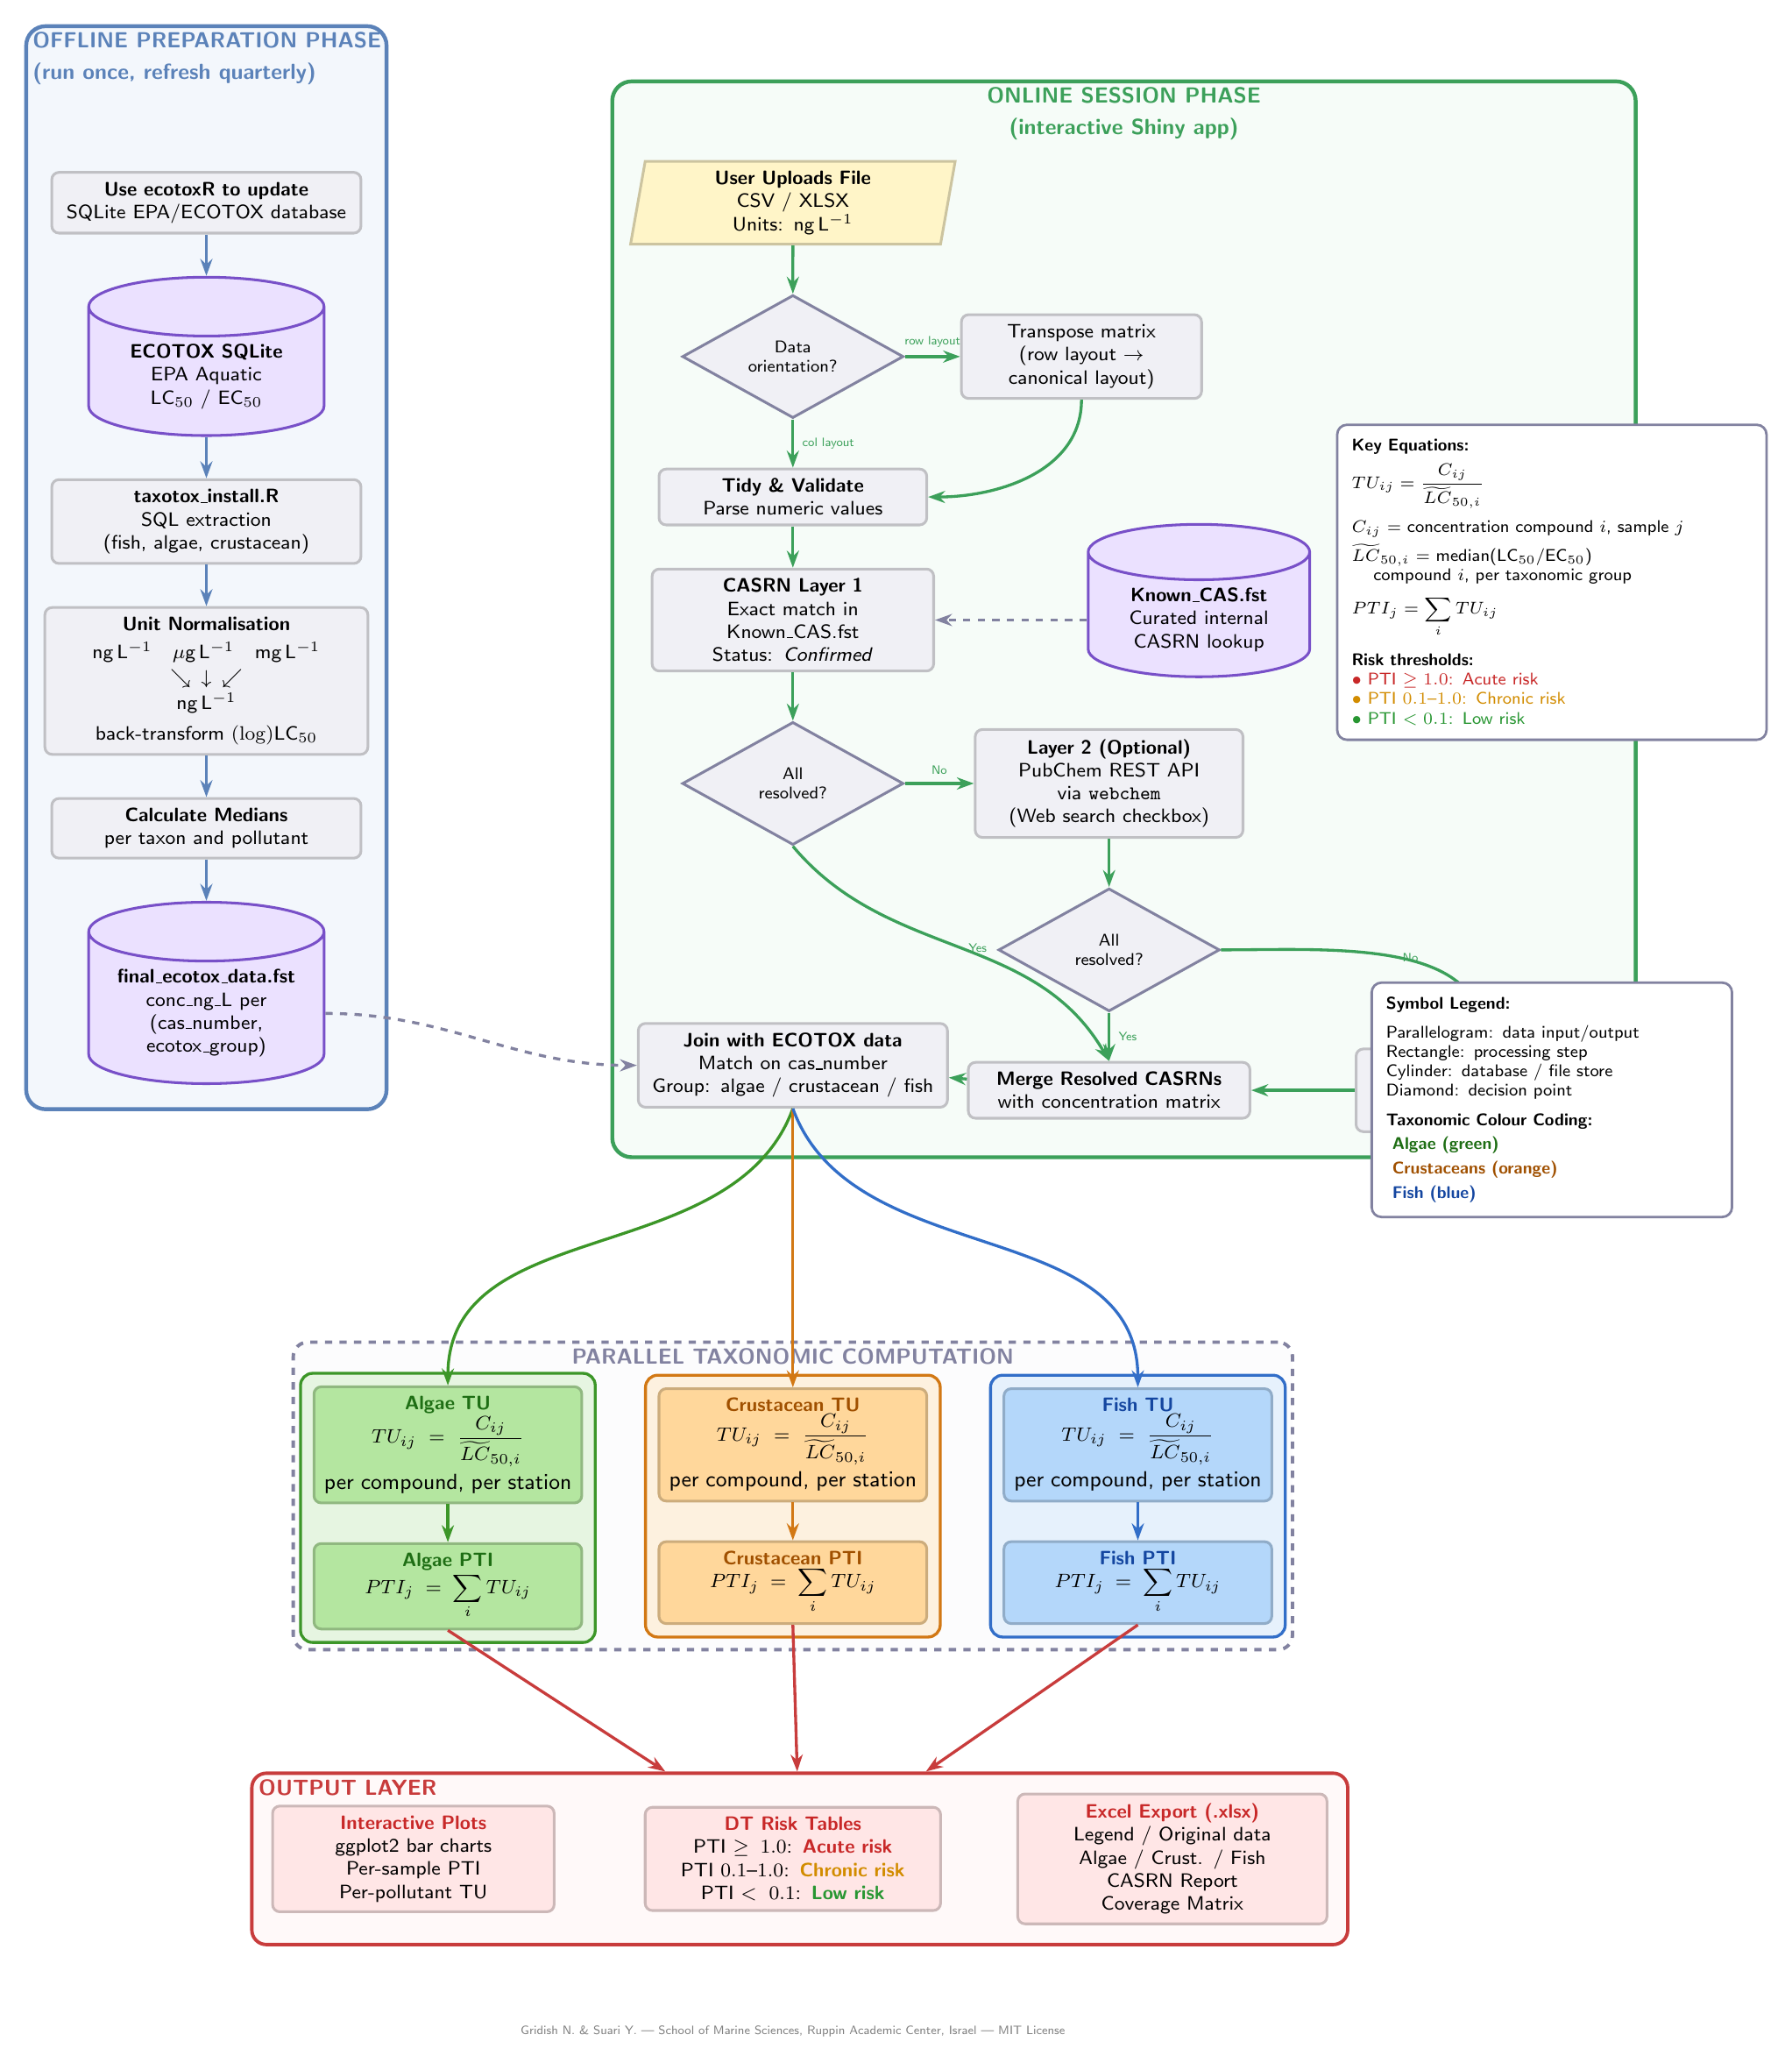
\begin{tikzpicture}[node distance=0.55cm and 0.55cm]

% Phantom nodes to extend box tops above first nodes, giving room for labels
\node[minimum size=0pt, inner sep=0pt] (offline_top) at (2.0, 2.2) {};
\node[minimum size=0pt, inner sep=0pt] (online_top)  at (10.5, 1.4) {};

%--- OFFLINE PHASE ---
\node[proc=ProcessGray, text width=4.2cm] (ecotox_dl) at (2.0,0)
  {\textbf{Use ecotoxR to update}\\SQLite EPA/ECOTOX database};

\node[db, below=0.6cm of ecotox_dl, text width=3.2cm] (sqlite)
  {\textbf{ECOTOX SQLite}\\EPA Aquatic\\LC$_{50}$ / EC$_{50}$};

\node[proc=ProcessGray, text width=4.2cm, below=0.6cm of sqlite] (install_r)
  {\textbf{taxotox\_install.R}\\SQL extraction\\(fish, algae, crustacean)};

\node[proc=ProcessGray, text width=4.4cm, below=0.6cm of install_r] (units)
  {\textbf{Unit Normalisation}\\[2pt]
   ng\,L$^{-1}$\quad$\mu$g\,L$^{-1}$\quad mg\,L$^{-1}$\\[1pt]
   $\searrow$\enspace$\downarrow$\enspace$\swarrow$\\[1pt]
   ng\,L$^{-1}$\\[3pt]
   back-transform $(\log)$LC$_{50}$};

\node[proc=ProcessGray, text width=4.2cm, below=0.6cm of units] (calc_medians)
  {\textbf{Calculate Medians}\\per taxon and pollutant};

\node[db, below=0.6cm of calc_medians, text width=3.2cm] (fst_ecotox)
  {\textbf{final\_ecotox\_data.fst}\\conc\_ng\_L per\\(cas\_number, ecotox\_group)};

%--- ONLINE PHASE ---
\node[data=InputColor, text width=4.0cm] (user_input) at (10.5, 0)
  {\textbf{User Uploads File}\\CSV / XLSX\\Units: ng\,L$^{-1}$};

\node[dec, below=0.7cm of user_input] (orient_dec)
  {Data\\orientation?};

\node[proc=ProcessGray, right=0.8cm of orient_dec, text width=3.2cm] (transpose)
  {Transpose matrix\\(row layout $\rightarrow$\\canonical layout)};

\node[proc=ProcessGray, below=0.7cm of orient_dec, text width=3.6cm] (tidy)
  {\textbf{Tidy \& Validate}\\Parse numeric values};

\node[proc=ProcessGray, below=0.6cm of tidy, text width=3.8cm] (layer1)
  {\textbf{CASRN Layer 1}\\Exact match in\\Known\_CAS.fst\\Status: \textit{Confirmed}};

\node[db, right=2.2cm of layer1, text width=3.0cm] (known_cas)
  {\textbf{Known\_CAS.fst}\\Curated internal\\CASRN lookup};

\node[dec, below=0.7cm of layer1] (resolved1)
  {All\\resolved?};

\node[proc=ProcessGray, right=1.0cm of resolved1, text width=3.6cm] (layer2)
  {\textbf{Layer 2 (Optional)}\\PubChem REST API\\via \texttt{webchem}\\(Web search checkbox)};

\node[dec, below=0.7cm of layer2] (resolved2)
  {All\\resolved?};

\node[proc=ProcessGray, below=0.7cm of resolved2, text width=3.8cm] (merge_cas)
  {\textbf{Merge Resolved CASRNs}\\with concentration matrix};

\node[proc=ProcessGray, right=1.5cm of merge_cas, text width=3.4cm] (manual)
  {\textbf{Manual CASRN Entry}\\CASRN Matching tab\\User assigns CASRNs};

\node[proc=ProcessGray, text width=4.2cm] (join_ecotox) at (10.5, -12.5)
  {\textbf{Join with ECOTOX data}\\Match on cas\_number\\Group: algae / crustacean / fish};

%--- TAXONOMIC BLOCKS ---
\node[minimum size=0pt, inner sep=0pt] (tax_top) at (10.5, -16.8) {};
\node[proc=AlgaeColor, text width=3.6cm] (tu_algae) at (5.5,-18.0)
  {\textcolor{AlgaeDark}{\textbf{Algae TU}}\\
   $TU_{ij} = \dfrac{C_{ij}}{\widetilde{LC}_{50,i}}$\\[2pt]
   \small per compound, per station};

\node[proc=AlgaeColor, text width=3.6cm, below=0.55cm of tu_algae] (pti_algae)
  {\textcolor{AlgaeDark}{\textbf{Algae PTI}}\\
   $PTI_{j} = \displaystyle\sum_{i} TU_{ij}$};

\node[proc=CrustColor, text width=3.6cm] (tu_crust) at (10.5,-18.0)
  {\textcolor{CrustDark}{\textbf{Crustacean TU}}\\
   $TU_{ij} = \dfrac{C_{ij}}{\widetilde{LC}_{50,i}}$\\[2pt]
   \small per compound, per station};

\node[proc=CrustColor, text width=3.6cm, below=0.55cm of tu_crust] (pti_crust)
  {\textcolor{CrustDark}{\textbf{Crustacean PTI}}\\
   $PTI_{j} = \displaystyle\sum_{i} TU_{ij}$};

\node[proc=FishColor, text width=3.6cm] (tu_fish) at (15.5,-18.0)
  {\textcolor{FishDark}{\textbf{Fish TU}}\\
   $TU_{ij} = \dfrac{C_{ij}}{\widetilde{LC}_{50,i}}$\\[2pt]
   \small per compound, per station};

\node[proc=FishColor, text width=3.6cm, below=0.55cm of tu_fish] (pti_fish)
  {\textcolor{FishDark}{\textbf{Fish PTI}}\\
   $PTI_{j} = \displaystyle\sum_{i} TU_{ij}$};

%--- OUTPUT LAYER ---
\node[proc=OutputColor, text width=3.8cm] (plots) at (5.0,-24.0)
  {\textcolor{RiskRed}{\textbf{Interactive Plots}}\\ggplot2 bar charts\\Per-sample PTI\\Per-pollutant TU};

\node[proc=OutputColor, text width=4.0cm] (tables) at (10.5,-24.0)
  {\textcolor{RiskRed}{\textbf{DT Risk Tables}}\\PTI $\geq 1.0$: \textcolor{RiskRed}{\textbf{Acute risk}}\\PTI $0.1$--$1.0$: \textcolor{RiskAmber}{\textbf{Chronic risk}}\\PTI $< 0.1$: \textcolor{RiskGreenC}{\textbf{Low risk}}};

\node[proc=OutputColor, text width=4.2cm] (excel) at (16.0,-24.0)
  {\textcolor{RiskRed}{\textbf{Excel Export (.xlsx)}}\\Legend / Original data\\Algae / Crust. / Fish\\CASRN Report\\Coverage Matrix};

%--- BACKGROUND CONTAINERS ---
\begin{scope}[on background layer]
\node[
  draw=OfflineBorder, line width=1.6pt,
  fill=OfflineBlue, fill opacity=0.35,
  rounded corners=8pt,
  fit=(offline_top)(ecotox_dl)(fst_ecotox)(calc_medians),
  inner sep=10pt,
  label={[seclabel=OfflineBorder,anchor=north west,align=left]north west:
    \textbf{OFFLINE PREPARATION PHASE}\\[2pt]\textit{(run once, refresh quarterly)}}
] (offline_box) {};

\node[
  draw=OnlineBorder, line width=1.6pt,
  fill=OnlineGreen, fill opacity=0.25,
  rounded corners=8pt,
  fit=(online_top)(user_input)(merge_cas)(transpose)(manual)(layer2),
  inner sep=10pt,
  label={[seclabel=OnlineBorder,anchor=north,align=center]north:
    \textbf{ONLINE SESSION PHASE}\\[2pt]\textit{(interactive Shiny app)}}
] (online_box) {};

\node[
  draw=ProcessBorder, line width=1.4pt, dashed,
  fill=ProcessGray, fill opacity=0.18,
  rounded corners=6pt,
  fit=(tax_top)(tu_algae)(pti_algae)(tu_crust)(pti_crust)(tu_fish)(pti_fish),
  inner sep=8pt,
  label={[seclabel=ProcessBorder,anchor=north,align=center]north:
    \textbf{PARALLEL TAXONOMIC COMPUTATION}}
] (tax_box) {};

\node[draw=AlgaeBorder,line width=1.2pt,fill=AlgaeColor,fill opacity=0.3,
  rounded corners=5pt,fit=(tu_algae)(pti_algae),inner sep=5pt] {};
\node[draw=CrustBorder,line width=1.2pt,fill=CrustColor,fill opacity=0.3,
  rounded corners=5pt,fit=(tu_crust)(pti_crust),inner sep=5pt] {};
\node[draw=FishBorder,line width=1.2pt,fill=FishColor,fill opacity=0.3,
  rounded corners=5pt,fit=(tu_fish)(pti_fish),inner sep=5pt] {};

\node[draw=OutputBorder,line width=1.4pt,fill=OutputColor,fill opacity=0.25,
  rounded corners=6pt,fit=(plots)(tables)(excel),inner sep=8pt,
  label={[seclabel=OutputBorder,anchor=north west]north west:\textbf{OUTPUT LAYER}}
] (output_box) {};
\end{scope}

%--- ARROWS ---
\draw[arr=OfflineBorder] (ecotox_dl) -- (sqlite);
\draw[arr=OfflineBorder] (sqlite) -- (install_r);
\draw[arr=OfflineBorder] (install_r) -- (units);
\draw[arr=OfflineBorder] (units.south) -- (calc_medians.north);
\draw[arr=OfflineBorder] (calc_medians.south) -- (fst_ecotox.north);

\draw[arr=ProcessBorder,dashed] (fst_ecotox.east) to[out=0,in=180] (join_ecotox.west);
\draw[arr=ProcessBorder,dashed] (known_cas.west) -- (layer1.east);

\draw[arr=OnlineBorder] (user_input) -- (orient_dec);
\draw[arr=OnlineBorder] (orient_dec) -- node[right,font=\tiny\sffamily]{col layout} (tidy);
\draw[arr=OnlineBorder] (orient_dec) -- node[above,font=\tiny\sffamily]{row layout} (transpose);
\draw[arr=OnlineBorder] (transpose.south) to[out=270,in=0] (tidy.east);
\draw[arr=OnlineBorder] (tidy) -- (layer1);
\draw[arr=OnlineBorder] (layer1) -- (resolved1);
\draw[arr=OnlineBorder] (resolved1.east) -- node[above,font=\tiny\sffamily]{No} (layer2.west);
\draw[arr=OnlineBorder] (resolved1.south) to[out=310,in=120] node[right,font=\tiny\sffamily]{Yes} (merge_cas.north);
\draw[arr=OnlineBorder] (layer2.south) -- (resolved2.north);
\draw[arr=OnlineBorder] (resolved2.south) -- node[right,font=\tiny\sffamily]{Yes} (merge_cas.north);
\draw[arr=OnlineBorder] (resolved2.east) to[out=0,in=90] node[right,font=\tiny\sffamily]{No} (manual.north);
\draw[arr=OnlineBorder] (manual.west) -- (merge_cas.east);
\draw[arr=OnlineBorder] (merge_cas) -- (join_ecotox);
\draw[arr=AlgaeBorder] (join_ecotox.south) to[out=250,in=90] (tu_algae.north);
\draw[arr=CrustBorder]  (join_ecotox.south) -- (tu_crust.north);
\draw[arr=FishBorder]   (join_ecotox.south) to[out=290,in=90] (tu_fish.north);

\draw[arr=AlgaeBorder] (tu_algae) -- (pti_algae);
\draw[arr=CrustBorder] (tu_crust) -- (pti_crust);
\draw[arr=FishBorder]  (tu_fish)  -- (pti_fish);

\draw[arr=OutputBorder] (pti_algae.south) -- (output_box);
\draw[arr=OutputBorder] (pti_crust.south) -- (output_box);
\draw[arr=OutputBorder] (pti_fish.south)  -- (output_box);

%--- FORMULA BOX ---
\node[
  draw=ProcessBorder, line width=1pt,
  fill=white, rounded corners=4pt,
  font=\scriptsize\sffamily,
  text width=5.8cm, align=left, inner sep=6pt
] at (21.5, -5.5) {
  \textbf{Key Equations:}\\[3pt]
  $TU_{ij} = \dfrac{C_{ij}}{\widetilde{LC}_{50,i}}$\\[4pt]
  $C_{ij}$ = concentration compound $i$, sample $j$\\[2pt]
  $\widetilde{LC}_{50,i}$ = median(LC$_{50}$/EC$_{50}$)\\
  \hspace*{1.2em}compound $i$, per taxonomic group\\[4pt]
  $PTI_{j} = \displaystyle\sum_{i} TU_{ij}$\\[6pt]
  \textbf{Risk thresholds:}\\
  \textcolor{RiskRed}{$\bullet$ PTI $\geq 1.0$: Acute risk}\\
  \textcolor{RiskAmber}{$\bullet$ PTI $0.1$--$1.0$: Chronic risk}\\
  \textcolor{RiskGreenC}{$\bullet$ PTI $< 0.1$: Low risk}
};

%--- LEGEND ---
\node[
  draw=ProcessBorder, line width=1pt,
  fill=white, rounded corners=4pt,
  font=\scriptsize\sffamily,
  text width=4.8cm, align=left, inner sep=6pt
] at (21.5, -13.0) {
  \textbf{Symbol Legend:}\\[4pt]
  Parallelogram: data input/output\\
  Rectangle: processing step\\
  Cylinder: database / file store\\
  Diamond: decision point\\[4pt]
  \textbf{Taxonomic Colour Coding:}\\[2pt]
  \textcolor{AlgaeDark}{$\blacksquare$} \textcolor{AlgaeDark}{\textbf{Algae (green)}}\\[2pt]
  \textcolor{CrustDark}{$\blacksquare$} \textcolor{CrustDark}{\textbf{Crustaceans (orange)}}\\[2pt]
  \textcolor{FishDark}{$\blacksquare$} \textcolor{FishDark}{\textbf{Fish (blue)}}
};

%--- ATTRIBUTION ---
\node[font=\tiny\sffamily, text=gray] at (10.5,-26.5)
  {Gridish N. \& Suari Y. --- School of Marine Sciences, Ruppin Academic Center, Israel --- MIT License};

\end{tikzpicture}
\end{center}
\end{document}
